
\subsection{The Theory of Hurricanes}
\label{sec:hurr-theory}
\subsubsection{The Carnot cyclone}
\label{sec:carnot}

The hurricane can be idealised as a Carnot cycle as in Figure~\ref{fig:hurricane-carnot},
as was originally proposed Kleinschmidt,~1951~\cite{kleinschmidt1951grundlagen},
and reproposed by Emanuel~1986~\cite{emanuel1986air, emanuel1987dependence, lilly1985steady,}.
\begin{figure}
\centering
    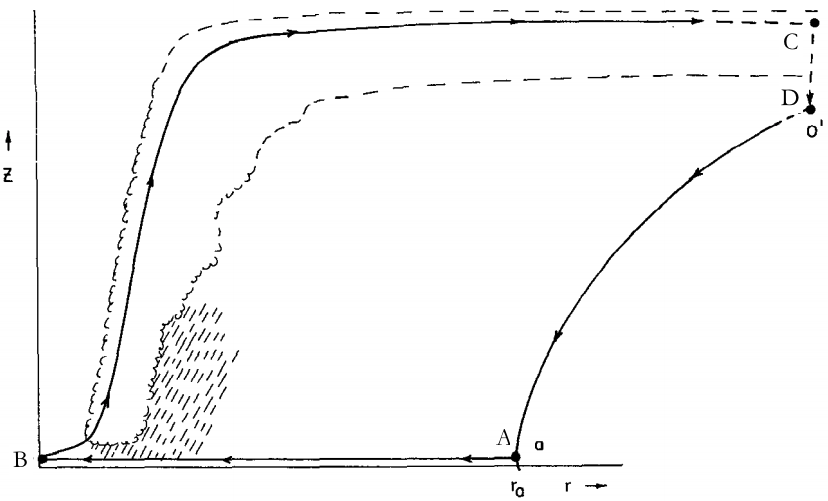
\includegraphics[width=\linewidth]{images/hurricane-carnot.png}\\
    \textit{Figure 1 from~\cite{emanuel1991theory}. }
    \caption{An idealised Carnot cycle where air parcels travel clockwise:
            A$\rightarrow$B travelling isothermally inwards into the eye-wall extracting enthalpy
            from the sea, and gaining entropy through kinetic energy dissipation;
            B$\rightarrow$C moist adiabatically thrust up into the stratosphere
            at the eye-wall and out to some some subsidence point;
            C$\rightarrow$D initial isothermal descent, albeit with some loss through radiation;
            D$\rightarrow$A final moist adiabatic descent~\cite{emanuel2018progress}. }
            \label{fig:hurricane-carnot}

\end{figure}



The temperature of the sea surface temperature controls the hurricane\cite{emanuel1991theory, emanuel2018progress}.



Hurricanes are a finite amplitude instability, and there is a
clear separation between a tropical storm and a hurricane~\cite{emanuel2005divine}.

As shown in Figure~\ref{fig:hurricane-carnot} Enthalpy is acquired from the sea surface,
and entropy from the dissipation of kinetic energy,
 as the air travels isothermally towards the eyewall.
 At the eyewall the air rises moist adiabatically
 to the lower stratosphere and out to some distance from the storm.
 In a simplified model it then subsides
 approximately isothermally at first, albeit with some loss through radiation.
 The final descent is approximately moist adiabatic~\cite{emanuel2018progress}.

This is nearly an ideal carnot cycle, this converts heat energy of the sea surface into
mechanical energy of the winds, doing the majority of the work against the sea surface.

The potential intensity (equation 15-7 in \cite{emanuel2018progress}) is,

\begin{equation}
\left|\mathbf{V}_{s}\right|^{2}=\frac{C_{k}}{C_{D}} \frac{T_{s}-T_{o}}{T_{o}}\left(k_{0}^{*}-k\right),
\tag{PI}
\label{eq:PI}
\end{equation}

where $C_d$ is the surface drag coefficient $C_k$ is the dimensionless
surface exchange coefficient for enthalpy.
$T_s$ is the sea surface temperature, $T_o$ is the temperature of the
lower stratosphere at the end of the moist adiabatic rise.
One can see that the a warmer sea surface, and a cooler lower stratosphere
would both lead to a higher potential intensity in paragraph~\cite{emanuel1991theory}.
Further in \ref{eq:PI} the enthalpy per unit mass (equation 15-8 in \cite{emanuel2018progress}) is

\begin{equation}
k \equiv c_{p} T+L_{v} q,
\label{eq:enthalpy_per_unit_mass}
\end{equation}

where $c_p$ is the heat capacity at constant pressure and $L_{v}$ is the latent heat
of vaporisation. $k_{0}^{*}$ is the saturation enthalpy at the sea surface.


There is a positive feedback loop from air cooling adiabatically as it flows down
the pressure gradient, and therefore increasing the enthalpy disequilibrium
$k_{0}^{*}-k$, leading to a root below 700 mbar central pressure called a `hypercane'.

The Carnot cycle derivation makes no assumption about hydrostatic of gradient
balance.

Therefore given the sea surface temperature, there is some maximum intensity
that a hurricane could reach given the rest of the climate \cite{bister2002low}.

The simplest

\cite{bister1996development,bister1998dissipative, bister2002low}

This makes some simplifying assumptions. One of the main reasons for
hurricanes failing to reach their potential intensity is that not all of the
water column at the temperature
of the surface, instead only up to some depth. The depth of warm water
is much larger at the western boundary currents~\cite{hogg1995western}, which means that if a hurricane
travels down the axis of the current (e.g. the loop current)
it can reach a higher intensity than
if it travelled 20km to one side.





\subsubsection{Cyclogenesis}


Given that there is a thermodynamic disequilibrium between the Ocean and
atmosphere, it is reasonable to ask why there are not more tropical cyclones
continuously spontaniously emerging.

Warm air rises in cumulonimbus clouds,
 dries, and then falls down very dry.
A decrease in humidity with altitude.
 Middle level dryness.
cumulonimbus clouds clump together.
 More updrafts give more rain.

Nascent cloud cluster dies away.


Middle atmosphere becomes humidified.

William grey cyclogenesis~\cite{gray1975tropical}.

African Easterly Waves.

Ordinary cold front that penetrates tropics.

Tropical cyclogenesis is one of the
 great mysteries of the tropical atmosphere.

An EC does not need anything to trigger it.

Notes from Emanuel~\cite{emanuel2005divine}.

There was a cold bias in CMIP5 models~\cite{camargo2013global}.


\begin{figure*}
\centering
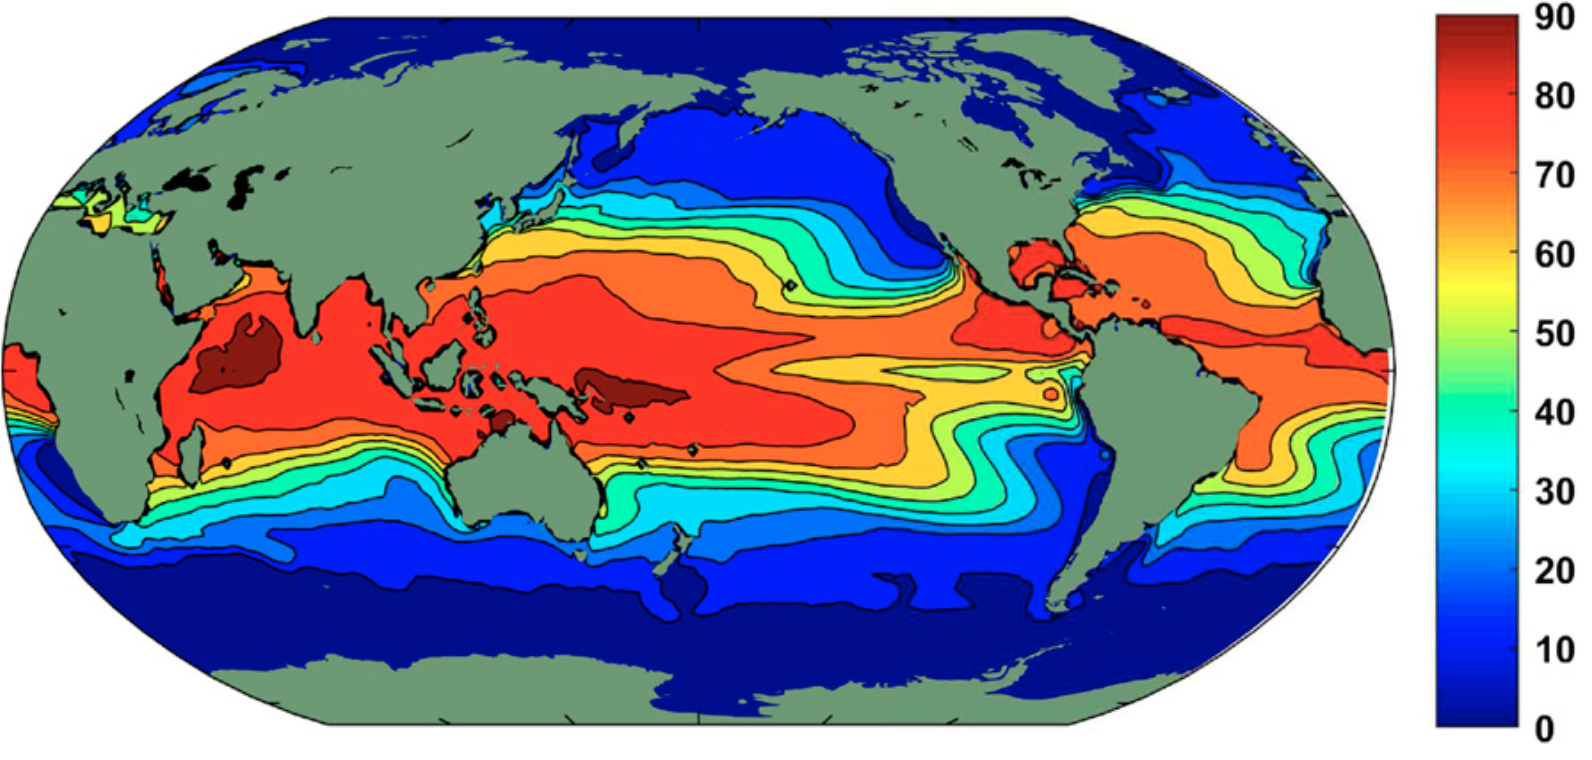
\includegraphics[width=\linewidth]{images/PI-max-year.png}\\
\textit{Figure 15-7 from \cite{emanuel2018progress}.}
\caption{The annual maximum of the potential intensity (m s$^{-1}$), calculated using
~\cite{bister2002low} and ERA-Interim data 1979-2016.
This is product maps on well to the block maxima procedure in §~\ref{sec:evt}.
}
\label{fig:eman}
\end{figure*}

